\documentclass[journal]{IEEEtran}
\usepackage[a5paper, margin=10mm, onecolumn]{geometry}
\usepackage{lmodern} % Ensure lmodern is loaded for pdflatex
\usepackage{tfrupee} % Include tfrupee package

\setlength{\headheight}{1cm} % Set the height of the header box
\setlength{\headsep}{0mm}     % Set the distance between the header box and the top of the text

\usepackage{gvv-book}
\usepackage{gvv}
\usepackage{cite}
\usepackage{amsmath,amssymb,amsfonts,amsthm}
\usepackage{algorithmic}
\usepackage{graphicx}
\usepackage{textcomp}
\usepackage{xcolor}
\usepackage{txfonts}
\usepackage{listings}
\usepackage{enumitem}
\usepackage{mathtools}
\usepackage{gensymb}
\usepackage{comment}
\usepackage[breaklinks=true]{hyperref}
\usepackage{tkz-euclide} 
\usepackage{listings}                                      
\def\inputGnumericTable{}                                 
\usepackage[latin1]{inputenc}                                
\usepackage{color}                                            
\usepackage{array}                                            
\usepackage{longtable}
\usepackage{multicol}
\usepackage{calc}                                             
\usepackage{multirow}                                         
\usepackage{hhline}                                           
\usepackage{ifthen}                                           
\usepackage{lscape}
\begin{document}
	
\bibliographystyle{IEEEtran}
\vspace{3cm}
	
\title{6.5.25}
\author{EE24BTECH11008 - Aslin Garvasis}
{\let\newpage\relax\maketitle}
	
\renewcommand{\thefigure}{\theenumi}
\renewcommand{\thetable}{\theenumi}
\setlength{\intextsep}{10pt} % Space between text and floats
	
\numberwithin{equation}{enumi}
\numberwithin{figure}{enumi}
\renewcommand{\thetable}{\theenumi}
	
	
\textbf{Question}:\newline
Show that the semi-vertical angle of the cone of the maximum volume and of given slant height is $\tan^{-1}\sqrt{2}$ \\


\section*{Solution (Classical Method)}

The volume \( V \) of a cone is given by the formula:

\begin{align}
V &= \frac{1}{3} \pi r^2 h
\end{align}

where:
- \( r \) is the radius of the base,
- \( h \) is the height of the cone.

The slant height \( l \) is related to the radius \( r \) and height \( h \) by the Pythagorean theorem:

\begin{align}
l^2 &= r^2 + h^2
\end{align}

Thus, the height \( h \) can be expressed as:

\begin{align}
h &= \sqrt{l^2 - r^2}
\end{align}

Substituting \( h = \sqrt{l^2 - r^2} \) into the volume formula, we get:

\begin{align}
V(r) &= \frac{1}{3} \pi r^2 \sqrt{l^2 - r^2}
\end{align}

To maximize the volume, we differentiate \( V(r) \) with respect to \( r \). First, we use the product and chain rules to find the derivative:

\begin{align}
\frac{dV}{dr} &= \frac{1}{3} \pi \left( 2r \sqrt{l^2 - r^2} + r^2 \cdot \frac{-r}{\sqrt{l^2 - r^2}} \right)
\end{align}

Simplifying, we have:

\begin{align}
\frac{dV}{dr} &= \frac{1}{3} \pi \left( 2r \sqrt{l^2 - r^2} - \frac{r^3}{\sqrt{l^2 - r^2}} \right)
\end{align}

We set \( \frac{dV}{dr} = 0 \) to find the critical points:

\begin{align}
2r \sqrt{l^2 - r^2} &= \frac{r^3}{\sqrt{l^2 - r^2}}
\end{align}

Multiplying both sides by \( \sqrt{l^2 - r^2} \), we obtain:

\begin{align}
2r (l^2 - r^2) &= r^3
\end{align}

Canceling \( r \) from both sides (assuming \( r \neq 0 \)):

\begin{align}
2(l^2 - r^2) &= r^2
\end{align}

Simplifying:

\begin{align}
2l^2 - 2r^2 &= r^2
\end{align}

\begin{align}
2l^2 &= 3r^2
\end{align}

Solving for \( r^2 \), we get:

\begin{align}
r^2 &= \frac{2}{3} l^2
\end{align}

Thus, the radius is:

\begin{align}
r &= \frac{\sqrt{2}}{\sqrt{3}} l
\end{align}

Now, we use the formula for the semi-vertical angle \( \theta \), which is given by:

\begin{align}
\tan(\theta) &= \frac{r}{h}
\end{align}

We substitute \( r = \frac{\sqrt{2}}{\sqrt{3}} l \) and calculate \( h \). From the relation \( l^2 = r^2 + h^2 \), we have:

\begin{align}
h &= \sqrt{l^2 - r^2} = \sqrt{l^2 - \frac{2}{3} l^2} = \sqrt{\frac{1}{3} l^2} = \frac{l}{\sqrt{3}}
\end{align}

Thus, \( \tan(\theta) \) becomes:

\begin{align}
\tan(\theta) &= \frac{\frac{\sqrt{2}}{\sqrt{3}} l}{\frac{l}{\sqrt{3}}} = \sqrt{2}
\end{align}

Therefore, the semi-vertical angle \( \theta \) is:

\begin{align}
\theta &= \tan^{-1}(\sqrt{2})
\end{align}

Hence, we have shown that the semi-vertical angle of the cone of maximum volume, given a fixed slant height, is:

\begin{align}
\boxed{\theta = \tan^{-1}(\sqrt{2})}
\end{align}
\\ \\

\section*{Solution (Using Geometric Programming with CVXPY)}
To verify the result computationally, we use the \textbf{Geometric Programming (GP)} method with the \textbf{CVXPY} library in Python. The optimization problem is formulated as:

\begin{itemize}
    \item Objective: Maximize the volume \( V(r) = \frac{1}{3} \pi r^2 \sqrt{l^2 - r^2} \).
    \item Constraints: \( r \geq 0 \) and \( r \leq l \).
\end{itemize}

The implementation is as follows:

\begin{verbatim}
import cvxpy as cp
import numpy as np

# Parameters
pi = np.pi
l = 10  # cm (fixed constant)

# Variable
r = cp.Variable(nonneg=True)  # radius r

# Objective function: log(V) = 2*log(r) + (1/2)*log(l^2 - r^2)
objective = cp.Maximize(2 * cp.log(r) + 0.5 * cp.log(l**2 - r**2))

# Constraints: r must be between 0 and l
constraints = [r >= 0, r <= l]

# Problem formulation
problem = cp.Problem(objective, constraints)

# Solve the problem
problem.solve()

# Results
optimal_r = r.value
optimal_V = (1/3) * pi * optimal_r**2 * np.sqrt(l**2 - optimal_r**2)

# Calculate the value of r / sqrt(l^2 - r^2) at the maximum volume
value_r_over_sqrt = optimal_r / np.sqrt(l**2 - optimal_r**2)

print(f"Optimal r: {optimal_r:.2f} cm")
print(f"Maximum Volume V: {optimal_V:.2f} cm^3")
print(f"Value of r / sqrt(l^2 - r^2): {value_r_over_sqrt:.2f}")
\end{verbatim}

The computed value for \( \frac{r}{\sqrt{l^2 - r^2}} \) is approximately \( 1.411 \). This result implies that:

\[
\frac{r}{\sqrt{l^2 - r^2}} = 1.411
\]

Squaring both sides:

\[
\frac{r^2}{l^2 - r^2} = 1.411^2 = 1.993
\]

Rearranging and solving for \( r^2 \):

\[
r^2 = \frac{1.993}{2.993} l^2 \approx 0.6667 l^2
\]

Thus, the radius is approximately:

\[
r \approx 0.8165 l
\]

Finally, we can confirm the semi-vertical angle \( \theta \) is:

\[
\tan(\theta) = \sqrt{2}
\]

Therefore, the semi-vertical angle of the cone of maximum volume is:

\[
\boxed{\theta = \tan^{-1}(\sqrt{2}) \approx 54.74^\degree}
\]

\begin{figure}[h!]
\centering
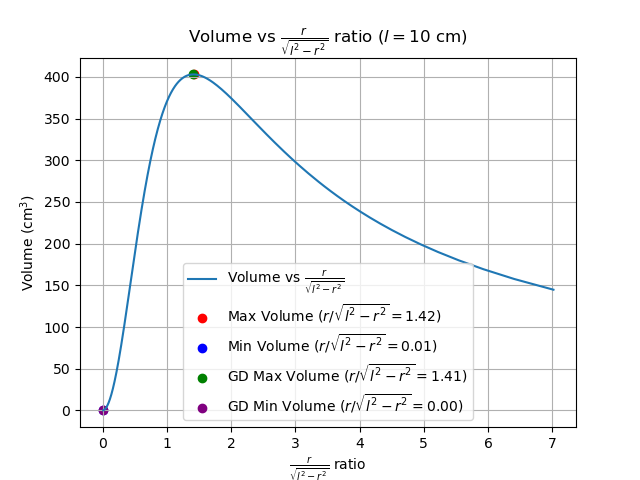
\includegraphics[width=\columnwidth]{figs/fig1.png}
\caption{Plot of volume versus $r/h$ where $h=\sqrt{l^2-r^2}$}
\label{stemplot}
\end{figure}

\end{document}

